%%%%%%%%%%%%%%%%%%%%%%%%%%%%%%%%%%%%%%%%%%%%%%%%%%%%%%%%%%%%%%%%%%%%%%%%%%%%%%%%
%
%  Project: Development of Security Protocols by Refinement
%
%  Module:  document/session_graph.tex (Isabelle/HOL 2016-1)
%  ID:      $Id: root.tex 134929 2017-05-24 18:27:58Z csprenge $
%  Author:  Christoph Sprenger, ETH Zurich <sprenger@inf.ethz.ch>
%  
%  session graph for PDF document
%
%  Copyright (c) 2009-2017 Christoph Sprenger 
%  Licence: LGPL
%
%%%%%%%%%%%%%%%%%%%%%%%%%%%%%%%%%%%%%%%%%%%%%%%%%%%%%%%%%%%%%%%%%%%%%%%%%%%%%%%%
\documentclass[11pt,a4paper]{report}
\usepackage[T1]{fontenc}
\usepackage{isabelle,isabellesym}

% input user-defined stuff
\usepackage{a4wide}
%*******************************************************************************
%
%  Project: Development of Security Protocols by Refinement  
%
%  Module: CryptoLib/document/isapreamble.tex
%  ID:     $Id: isapreamble.tex 134924 2017-05-24 17:23:15Z csprenge $
%  Author:  Christoph Sprenger, ETH Zurich <sprenger@inf.ethz.ch>
%
%  definitions for LaTeX documents generated by Isabelle
%
%  Copyright (C) 2009 Christoph Sprenger 
%  Licence: LGPL
%
%*******************************************************************************)


% additional packages
\usepackage{graphicx}       % to display session graph


% further packages required for unusual symbols (see also
% isabellesym.sty), use only when needed

%\usepackage{amssymb}
  %for \<leadsto>, \<box>, \<diamond>, \<sqsupset>, \<mho>, \<Join>,
  %\<lhd>, \<lesssim>, \<greatersim>, \<lessapprox>, \<greaterapprox>,
  %\<triangleq>, \<yen>, \<lozenge>

%\usepackage[greek,english]{babel}
  %option greek for \<euro>
  %option english (default language) for \<guillemotleft>, \<guillemotright>

%\usepackage[utf8]{inputenc}
  %for \<onesuperior>, \<onequarter>, \<twosuperior>, \<onehalf>,
  %\<threesuperior>, \<threequarters>, \<degree>

%\usepackage[only,bigsqcap]{stmaryrd}
  %for \<Sqinter>

%\usepackage{eufrak}
  %for \<AA> ... \<ZZ>, \<aa> ... \<zz> (also included in amssymb)

%\usepackage{textcomp}
  %for \<cent>, \<currency>

% this should be the last package used
\usepackage{pdfsetup}

% urls in roman style, theory text in math-similar italics
\urlstyle{rm}
\isabellestyle{it}


\begin{document}

\title{Development of Security Protocols by Refinement}
\author{Christoph Sprenger and Ivano Somaini \\[.5ex]
ETH Zurich, Switzerland}
\maketitle

\begin{abstract}
We propose a development method for security protocols based on stepwise refinement. Our refinement strategy transforms abstract security goals into protocols that are secure when operating over an insecure channel controlled by a Dolev-Yao-style intruder. As intermediate levels of abstraction, we employ messageless guard protocols and channel protocols communicating over channels with security properties. These abstractions provide insights on why protocols are secure and foster the development of families of protocols sharing common structure and properties. We have implemented our method in Isabelle/HOL and used it to develop different entity authentication and key establishment protocols, including realistic features such as key confirmation, replay caches, and encrypted tickets. Our development highlights that guard protocols and channel protocols provide fundamental abstractions for bridging the gap between security properties and standard protocol descriptions based on cryptographic messages. It also shows that our refinement approach scales to protocols of nontrivial size and complexity.
\end{abstract}

\tableofcontents

% sane default for proof documents
\parindent 0pt\parskip 0.5ex

% display the theory dependency graph
%%%%%%%%%%%%%%%%%%%%%%%%%%%%%%%%%%%%%%%%%%%%%%%%%%%%%%%%%%%%%%%%%%%%%%%%%%%%%%%%
%
%  Project: Sumcheck Protocol 
%
%  Authors:  Azucena Garvia <zucegb@gmail.com>
%		   Christoph Sprenger <sprenger@inf.ethz.ch>
%		   Jonathan Bootle <jbt@zurich.ibm.com>
%  
%%%%%%%%%%%%%%%%%%%%%%%%%%%%%%%%%%%%%%%%%%%%%%%%%%%%%%%%%%%%%%%%%%%%%%%%%%%%%%%%

\begin{figure}[p]
  \begin{center}
    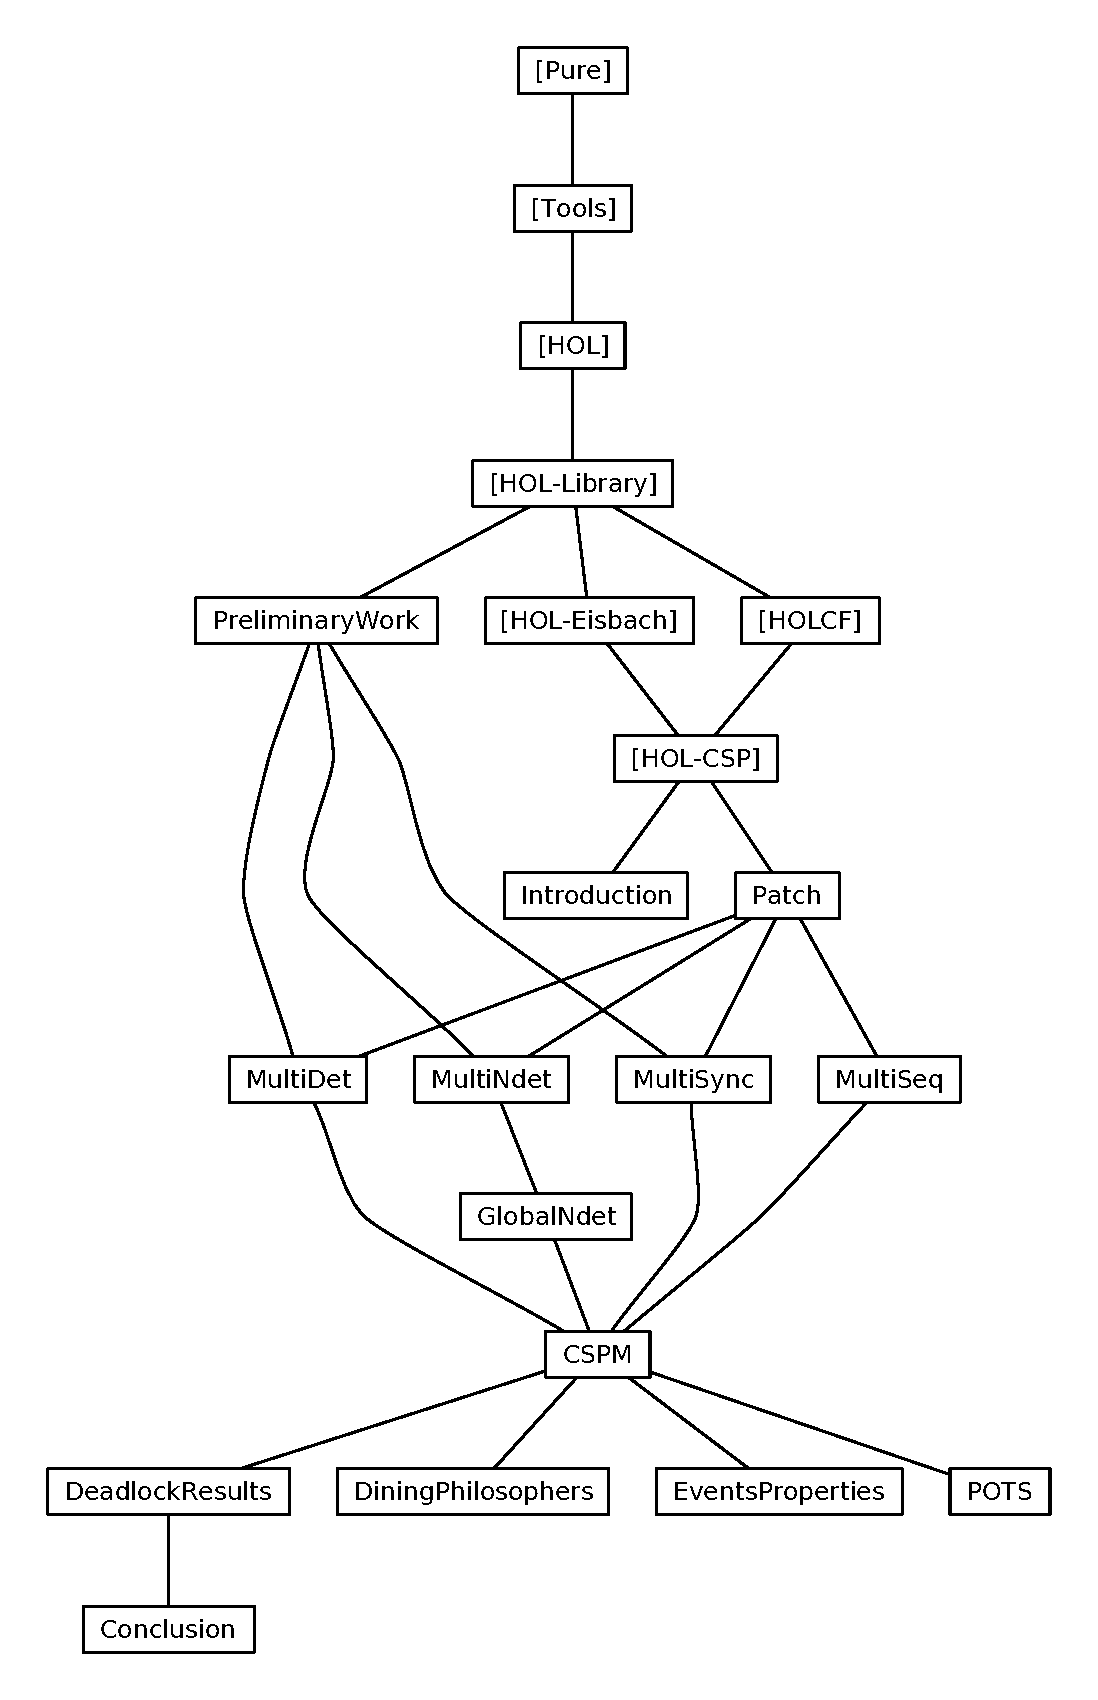
\includegraphics[scale=.7]{session_graph.pdf}
    \caption{Theory dependencies}
  \end{center}
  \label{fig:theory-dependencies}
\end{figure}



\section*{Preamble}

\subsection*{Related Publications}

The following papers describe our results in more detail:
\begin{itemize}
\item Christoph Sprenger and David Basin,
  \emph{Developing Security Protocols by Refinement}, CCS 2010.

\item Christoph Sprenger and David Basin,
  \emph{Refining Key Establishment}, CSF 2012.

\item Christoph Sprenger and David Basin,
  \emph{Refining Security Protocols},
  Journal of Computer Security (in submission), 2017.
\end{itemize}
  
Note: The Isabelle/HOL sources in this distribution also include the treatment
of session key compromise. This is described in our journal paper (see above), 
which subsumes the CCS 2010 and CSF 2012 papers.

\subsection*{Mapping the model names in our papers to the Isabelle/HOL theories}

For the sake of the presentation, the papers use shorter names for the models 
than the Isabelle theories.  Here is a mapping of the names. On the left you 
find the model name used in the papers and on the right the corresponding
Isabelle/HOL theory name. Note that the Isabelle theories contain a 
separate lemma or theorem for each invariant and refinement result.

\begin{description}
\item[Level 0] \mbox{ }
\begin{verbatim}
          Refinement/
  s0         s0g_secrecy   		  
  a0n        a0n_agree             
  a0i        a0i_agree             
\end{verbatim}

\item[Level 1] \mbox{ }
\begin{verbatim}
          Auth_simple/
  a1         m1_auth

          Key_establish/
  kt1        m1_keydist            
  kt1in      m1_keydist_iirn       
  kt1nn      m1_keydist_inrn
  nssk1      m1_nssk
  krb1       m1_kerberos 
  ds1        m1_ds
\end{verbatim}

\item[Level 2] \mbox{ }
\begin{verbatim}
          Auth_simple/
  a2         m2_auth_chan
  c2         m2_confid_chan

          Key_establish/  				
  nssk2      m2_nssk
  krb2       m2_kerberos 
  ds2        m2_ds
\end{verbatim}

\item[Level 3] \mbox{ }
\begin{verbatim}
          Auth_simple/
  iso3       m3_sig
  nsl3       m3_enc
  
          Key_establish/  				
  nssk3d     m3_nssk_par
  nssk3      m3_nssk
  krb3d      m3_kerberos_par
  krb3v      m3_kerberos5  
  krb3iv     m3_kerberos4  
  ds3d       m3_ds_par
  ds3        m3_ds
\end{verbatim}
\end{description}


% generated text of all theories
\input{session}

% optional bibliography
\bibliographystyle{abbrv}
\bibliography{root}

\end{document}

